% !TEX root = ../../../under-spec-z.tex

\subsection{The faithfully flat topology} % (fold)
\label{sub:the_faithfully_flat_topology}

    \emph{Throughout this section $\smc$ is a cosmos\footnote{
            In keeping with Hypothèse 2.6, \S2.2, p.14; recalling \cref{df:cosmos}.
        } and we use $\dcat$ to refer to an arbitrary category.}
    % We start this section by introducing a fundamental definition -- that of an \emph{affine scheme over a cosmos}.
    \emph{The structure of this section is largely based on \cite[\S1.2,~1.3]{Marty:2009tj} (where all proofs can be found) and \cite[\S1.1]{Toen:2008wy}.}

    \begin{definition}[Affine schemes over $\ccat$ {(Définition 2.7, \S2.2, p.14)}]\label{df:old-affine-schemes}
        The category of \emph{affine schemes over $\ccat$} is the opposite category
        \begin{equation*}
            \aff{\ccat}=\op{\comm{\ccat}}.
        \end{equation*}
        For an object $A\in\comm{\ccat}$ we write $\spec A$ to denote the corresponding object in $\aff{\ccat}$.
    \end{definition}

    % \subsubsection{Introduction to changes of base} % (fold)
    % \label{ssub:introduction_to_changes_of_base}

    %     \begin{definition}[Slice category]\label{df:slice-category}
    %         Let $\dcat$ be some category and $X\in\dcat$ some object.
    %         We define the \emph{slice category $\dcat/X$} (sometimes called the \emph{over category} and sometimes written \emph{$\dcat\downarrow X$}) as having
    %         \begin{itemize}
    %             \item \emph{objects:} morphisms $Y\to X$ in $\dcat$ for some $Y\in\dcat$;
    %             \item \emph{morphisms:} morphisms $Y\to Y'$ in $\dcat$ such that
    %                 \begin{equation*}
    %                     \begin{tikzcd}[column sep=1em]
    %                         Y \arrow[dr] \arrow[rr] & & Y' \arrow[dl]\\
    %                          & X & \\
    %                     \end{tikzcd}
    %                 \end{equation*}
    %                 commutes.\qedhere
    %         \end{itemize}
    %     \end{definition}

    %     Dually, we have the the \emph{coslice} (or \emph{under}) category $X/\dcat$: its objects are morphisms $X\to Y$, and its morphisms are morphisms $Y\to Y'$ making the induced triangle commute.
    %     Since the only difference between slice and coslice categories is the direction of the arrows, it makes sense to think that there might be some relation between the two in terms of opposite categories.
    %     The following lemma makes this relation explicit, and although we have no use for it at the moment, it proves useful later on.

    %     \begin{lemma}\label{le:op-coslice-slice}
    %         Let $\dcat$ be some category and $X\in\dcat$.
    %         Then $\op{(X/\dcat)} \cong \op{\dcat}/X$.
    %     \end{lemma}

    %     \begin{proof}
    %         TJH todo
    %     \end{proof}

    %     TJH mention what \cref{le:op-coslice-slice} means for functors!

    %     Once again, we now introduce a purely category-theoretic notion which we will later apply to our scenario.

    %     \begin{definition}[Change of base]
    %         Let $\dcat$ be a category with pullbacks, and $f\colon X\to Y$ a morphism in $\dcat$.
    %         Then the \emph{change of base functor $f^*\colon \dcat/Y\to\dcat/X$} is the induced functor given, on objects, by the pullback along $f$:
    %         \begin{equation*}
    %             \left(
    %                 \begin{tikzcd}
    %                     X' \arrow[d, "p"]\\
    %                     Y
    %                 \end{tikzcd}
    %             \right)
    %             \mapsto
    %             \left(
    %                 \begin{tikzcd}
    %                     X\prescript{f}{}{\times}^p_Y X' \arrow[d, "\pi_X"]\\
    %                     X
    %                 \end{tikzcd}
    %             \right)
    %         \end{equation*}
    %         and we write $p^*=f^*(p)=\pi_X$.
    %     \end{definition}

    % % subsubsection introduction_to_changes_of_base (end)


    \subsubsection{Commutative algebras} % (fold)
    \label{ssub:commutative_algebras}

        \begin{definition}[Commutative $A$-algebras]
            Let $A\in\comm{\ccat}$.
            The objects of $A/\comm{\ccat}$ are called \emph{commutative $A$-algebras}, and we write $\algc{A}$ to mean the category of such objects.
        \end{definition}

        This slightly opaque definition is best explained after showing how we can endow $\modc{A}$ with a symmetric monoidal structure.

        \begin{definition}[Coequaliser]\label{df:coequaliser}
            The \emph{coequaliser $\coeq(X\rightrightarrows Y)$} of two morphisms $f,g\colon X\to Y$ in $\dcat$ is defined by the universal property of being a pair $(Q,q)$, where $Q\in\dcat$ and $q\colon Y\to Q$, such that $q\circ f=q\circ g$, and for any other such pair $(R,r)$ there exists a unique morphism $\varphi\colon Q\to R$ such that the following diagram commutes:
            \begin{equation*}
                \begin{tikzcd}
                    X \arrow[r, shift left=.75ex, "f"] \arrow[r, shift right=.75ex, swap, "g"] & Y \arrow[r, "q"] \arrow[dr, "r"] & Q \arrow[d, dotted, "\varphi"]\\
                     & & R
                \end{tikzcd}
            \end{equation*}
        \end{definition}
        \vspace{-3em}
        \begin{definition}[Symmetric monoidal structure on $\modc{A}$]\label{df:smc-on-a-mod}
            Let $A\in\comm{\ccat}$.
            Define the bifunctor $(\blank\otimes_A\blank)\colon\modc{A}\times\modc{A}\to\modc{A}$ by the object of the coequaliser
            \begin{equation*}
                X\otimes_A Y = \coeq(X\otimes A\otimes Y\rightrightarrows X\otimes Y),
            \end{equation*}
            where the morphisms are the natural ones, namely
            \begin{align*}
                X\otimes (A\otimes Y) &\xrightarrow{\id_X\otimes\sigma_Y} X\otimes Y\\
                (X\otimes A)\otimes Y &\xrightarrow{(\sigma_X\circ\gamma_{XA})\otimes\id_Y} X\otimes Y.
            \end{align*}
            Then $(\modc{A},\otimes_A,A)$ is a symmetric monoidal category\footnote{
                \cite[Proposition~1.2.15,~\S1.2,~p.14]{Marty:2009tj}
            }.
        \end{definition}

        \begin{lemma}[Equivalent definitions of $\algc{A}$]\label{le:two-definitions-of-alg}
            Let $A\in\comm{\ccat}$.
            Then we have the equivalence of categories
            \begin{equation*}
                \comm{\modc{A}} \equiv \algc{A} = A/\comm{\ccat}
            \end{equation*}
            (using the symmetric monoidal structure from \cref{df:smc-on-a-mod}).
        \end{lemma}

        \begin{proof}
            \cite[Proposition~1.2.15,~\S1.2,~p.14]{Marty:2009tj}.
        \end{proof}

        Because of this equivalence we sometimes write objects of $\algc{A}$ as $X$ for some $X\in\comm{\modc{A}}$, and sometimes as $(A\to X)$ for some $X\in\comm{\ccat}$.
        Object-wise, we can think of the structures we have defined as follows:
        \begin{equation*}
            \comm{\modc{A}}\equiv\algc{A}\subset\modc{A}\subset\comm{\ccat}\subset\ccat.
        \end{equation*}

        % \begin{lemma}\label{le:commcatt-and-modca-bicomplete}
        %     Both $\comm{\ccat}$ and $\modc{A}$ are bicomplete, for all $A\in\comm{\ccat}$.
        % \end{lemma}

        % \begin{proof}
        %     \cite[Proposition~1.2.14,~\S1.2,~p.11]{Marty:2009tj}
        % \end{proof}

        % \begin{lemma}\label{le:modc-a-is-closed}
        %     Let $A\in\comm{\ccat}$.
        %     Then $(\modc{A},\otimes_A,A)$ is a closed symmetric monoidal category.
        % \end{lemma}

        % \begin{proof}
        %     \cite[Proposition~1.2.17,~\S1.2,~p.17]{Marty:2009tj}
        % \end{proof}

        \begin{corollary}\label{le:modc-a-cosmos-algc-a-bicomplete}
            Let $A\in\comm{\ccat}$.
            Then
            \begin{enumerate}[(i)]
                \item $\comm{\ccat}$ and $\algc{A}$ are bicomplete;
                \item $(\modc{A},\otimes_A,A)$ is a cosmos.\qedhere
            \end{enumerate}
        \end{corollary}

        \begin{proof}
            \cref{le:two-definitions-of-alg} and \cite[Propositions~1.2.14,~1.2.17~\S1.2]{Marty:2009tj}.
        \end{proof}

        \begin{lemma}\label{le:otimes-is-sqcup}
            Let $A\in\comm{\ccat}$ and $X,Y\in\comm{\modc{A}}$.
            Then
            \begin{equation*}
                X\otimes_A Y\cong X\sqcup_A Y
            \end{equation*}
            where the coproduct is taken in $\comm{\ccat}$.
        \end{lemma}

        \begin{proof}
            \cite[Proposition~1.2.6,~\S1.2,~p.16]{Marty:2009tj}
        \end{proof}
    
    % subsubsection commutative_algebras (end)


    \subsubsection{Change of base for modules over a monoid} % (fold)
    \label{ssub:change_of_base_for_modules_over_a_monoid}

        Assume we have some morphism $f\colon\spec B\to\spec A$ in $\aff{\ccat}$.
        We claim that this induces a forgetful functor $\modc{B}\to\modc{A}$.
        That is, on the level of objects, $\modc{B}\subset\modc{A}$.

        Take some object $X\in\modc{B}$.
        This comes with a $B$-action $\sigma_B\colon B\otimes X\to X$.
        We can compose $f$ and $\sigma_B$ to obtain
        \begin{equation*}
            \sigma_A\colon A\otimes X \xrightarrow{f\otimes\id_X} B\otimes X \xrightarrow{\sigma_B} X.
        \end{equation*}
        We claim that this is an $A$-action on $X$.
        This just means showing that both of the diagrams in \cref{df:module-over-monoid} commute.
        Here we show just one since the other is equally straightforward.
        Note that
        \begin{equation*}
            \begin{tikzcd}[row sep=2em,column sep=1em]
                1\otimes X \arrow[rr, "\eta_A\otimes\id_X"] \arrow[dr, swap, "\lambda_X"] & & A\otimes X \arrow[dl, "\sigma_A"]\\
                 & X &
            \end{tikzcd}
            =
            \begin{tikzcd}[row sep=2em,column sep=1em]
                1\otimes X \arrow[rr, "(f\circ\eta_A)\otimes\id_X"] \arrow[dr, swap, "\lambda_X"] & & B\otimes X \arrow[dl, "\sigma_B"]\\
                 & X &
            \end{tikzcd}
        \end{equation*}
        But $f$ is a morphism in $\comm{\ccat}$, so \mbox{$f\circ\eta_A=\eta_B$} (recall \cref{df:comm-c}), and hence the second diagram commutes.
        Thus so too does the first diagram.
        We also have an induced forgetful functor $\algc{B}\to\algc{A}$, since if $(B\to X)\in\algc{B}$ then, composing with $f$, we get $(A\to B\to X)\in\algc{A}$.
        
        We mention the forgetful functor $\modc{B}\to\modc{A}$ because it has a left-adjoint, namely
        \begin{equation*}
            (\blank\otimes_A B)\colon\modc{A}\to\modc{B}
        \end{equation*}
        (which is well defined: $f$ lets us consider $B$, which is a $B$-module, as an $A$-module).
        This tells us that $(\blank\otimes_A B)$ is right exact.


        % The functor $(\blank\otimes_A B)\colon\modc{A}\to\modc{B}$ also arises naturally in another way though: it is the change of base functor in $\aff{\ccat}$.
        % To see this, start again with some morphism $f\colon\spec B\to\spec A$ in $\aff{\ccat}$.
        % Then the change of base functor
        % \begin{align*}
        %     f^*\colon \aff{\ccat}/\spec A &\longrightarrow \aff{\ccat}/\spec B\\[1em]
        %     \left(
        %         \begin{array}{c}
        %             X\\
        %             \downarrow\\
        %             \spec A
        %         \end{array}
        %     \right) &\mapsto
        %     \left(
        %         \begin{array}{c}
        %             \spec B\times_{\spec A} X\\
        %             \downarrow\\
        %             \spec B
        %         \end{array}
        %     \right)
        % \end{align*}
        % is tautologically equivalent to the functor
        % \begin{align*}
        %     f^*\colon \op{\comm{\ccat}}/A &\longrightarrow \op{\comm{\ccat}}/B\\[1em]
        %     \left(
        %         \begin{array}{c}
        %             X\\
        %             \downarrow\\
        %             A
        %         \end{array}
        %     \right) &\mapsto
        %     \left(
        %         \begin{array}{c}
        %             B\times_A X\\
        %             \downarrow\\
        %             B
        %         \end{array}
        %     \right)\\
        % \end{align*}
        % which is equivalent to the functor
        % \begin{align*}
        %     g^*\colon A/\comm{\ccat} &\longrightarrow B/\comm{\ccat}\\[1em]
        %     \left(
        %         \begin{array}{c}
        %             A\\
        %             \downarrow\\
        %             X
        %         \end{array}
        %     \right) &\mapsto
        %     \left(
        %         \begin{array}{c}
        %             B\\
        %             \downarrow\\
        %             B\sqcup_A X
        %         \end{array}
        %     \right)
        % \end{align*}
        % by \cref{le:op-coslice-slice}.

        % Now $B\sqcup_A X\cong X\sqcup_A B$ (\textbf{TJH PROVE THIS or at least say why}), and both $A$ and $X$ are $B$-algebras (since we have, by definition, morphisms to both from $B$).
        % So \cref{le:otimes-is-sqcup} tells us that the change of base functor
        % \begin{equation*}
        %     f^*\colon\aff{\ccat}/\spec A\to\aff{\ccat}/\spec B
        % \end{equation*}
        % is simply
        % \begin{equation*}
        %     (\blank\otimes_A B)\colon\modc{A}\to\modc{B}
        % \end{equation*}
        % (after using the forgetful functor $\algc{A}=A/\comm{\ccat}\to\comm{\ccat}$).

        % \emph{TJH extending from $\algc{A}$ to $\modc{A}$?}
        
        % \textbf{TJH i am not really very certain about all of this -- check!}
    
    % subsubsection change_of_base_for_modules_over_a_monoid (end)


    \subsubsection{fpqc topology} % (fold)
    \label{ssub:fpqc_topology}
    
        Now we apply the results from \cref{ssub:commutative_algebras,ssub:change_of_base_for_modules_over_a_monoid}.
        Let $\tcat=\aff{\ccat}$ and, using $\op{(\aff{\ccat})}=\comm{\ccat}$, define the pseudofunctor
        \begin{align}\label{eq:m-and-d-for-fpqc}
            M\colon\op{(\aff{\ccat})}&\to\Cat\\[.35em]
            A&\mapsto\modc{A}\nonumber\\
            (A\to B)&\mapsto(\blank\otimes_A B\colon\modc{A}\to\modc{B}).\nonumber
        \end{align}
        We claim that $\tcat$ and $M$ satisfy the conditions of \cref{df:m-t-grothendieck-setup}, and so generate a Grothendieck topology on $\aff{\ccat}$.
        There are four conditions that we need to check\footnote{
            Really, we also need to check that $M$ actually \emph{is} a pseudofunctor, but since we only gave a rough definition of pseudofunctors we simply claim that this is, in fact, true.
        }:
        \begin{enumerate}[(i)]
            \item \emph{$\aff{\ccat}$ has finite limits}: \cref{le:modc-a-cosmos-algc-a-bicomplete} (recall that $\aff{\ccat}=\op{\comm{\ccat}}$);
            \item \emph{$\modc{A}$ is bicomplete}: \cref{le:modc-a-cosmos-algc-a-bicomplete};
            \item \emph{$(\blank\otimes_A B)$ has a conservative right adjoint}: the right adjoint is the forgetful functor $\modc{B}\to\modc{A}$, and this is conservative since it gives us $\modc{B}$ as a full subcategory of $\modc{A}$;
            \item \emph{the Beck-Chevalley condition}\footnote{
                This is proved (much more generally) in \cite[Example~2.35]{Shulman:2013tx}.
            }: say we have the following pullback diagram
            \begin{equation*}
                \begin{tikzcd}[row sep=.7em]
                     & \spec B \arrow[dr, "q"] &\\
                    \spec X \arrow[ur, "p'"] \arrow[dr, swap, "q'"] & & \spec C\\
                     & \spec A \arrow[ur, swap, "p"] &
                \end{tikzcd}
            \end{equation*}
            in $\aff{\ccat}$ (i.e. $\spec X=\spec B\times_{\spec C}\spec A$ is the pullback).
            Then $X=B\sqcup_C A$ is the pushout in $\comm{\ccat}$, and $A,B\in\comm{\modc{C}}\equiv\algc{C}$.
            \Cref{le:otimes-is-sqcup} then tells us that $X\cong B\otimes_C A$.
            Thus\footnote{
                The second isomorphism comes from associativity; the third comes from the fact that $M\otimes_B B\cong M$.
                Both these facts mirror the usual case of tensor products over a commutative ring, and can be proved by using \cref{le:otimes-is-sqcup}: $X\otimes_A Y\cong X\sqcup_A Y$.
            }, for $M\in\modc{B}$,
            \begin{equation*}
                M\otimes_B X \cong M\otimes_B(B\otimes_C A) \cong (M\otimes_B B)\otimes_C A \cong M\otimes_C A,
            \end{equation*}
            and so $p^*q_*=(\blank\otimes_C A)\cong(\blank\otimes_B X)=(q')_*(p')^*$.
        \end{enumerate}

        \begin{figure}[h]
            \centering
            \frame{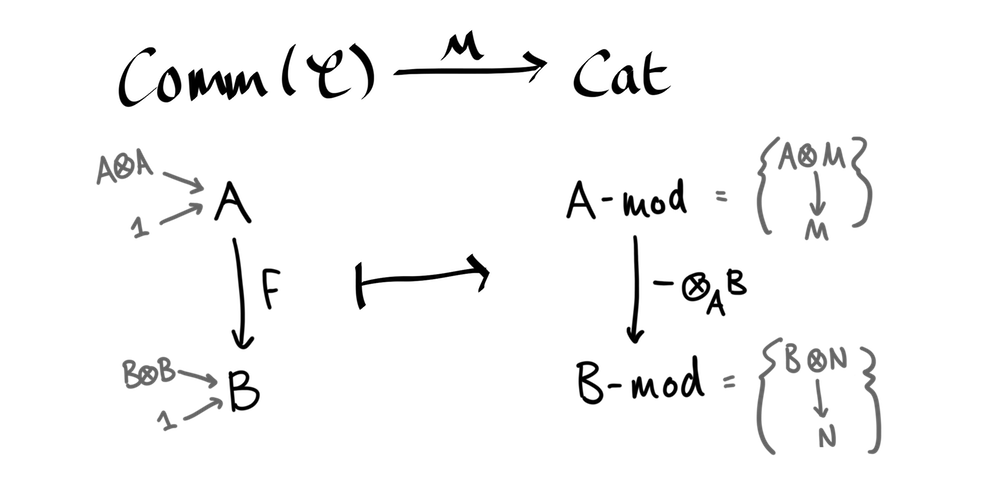
\includegraphics[width=.9\textwidth]{images/MfaithfullyflatwithAmod.png}}
            \caption{Constructing the fpqc topology -- compare with \cref{fg:grothendieckpseudofunctor}}
            \label{fg:MfaithfullyflatwithAmod}
        \end{figure}

        \begin{definition}[Faithfully flat and quasi-compact topology {(Définition~2.8, \S2.2, p.15)}]\label{df:fpqc-topology}
            With definitions as in \cref{eq:m-and-d-for-fpqc}, the $M$-faithfully flat topology on $\aff{\ccat}$ is called the \emph{faithfully flat and quasi-compact} (or simply \emph{fpqc}\footnote{
                In keeping with most current literature, we choose to keep the original French initialism rather than using the English \emph{ffqc}.
            }, or even just \emph{flat}) topology.
        \end{definition}

        \begin{note}[Change of base]\label{nt:change-of-base}
            For a morphism $f\colon X\to Y$ in some category $\dcat$ we have the notion of the \emph{change of base functor $f^*\colon\dcat/Y\to\dcat/X$} given by the pullback along $f$.
            This is \emph{not} quite what we mean when we call $(\blank\otimes_A B)$ a \emph{change of base}.
            We are instead applying the terminology from \cref{df:m-t-grothendieck-setup}: say we have
            \begin{equation*}
                \begin{tikzcd}[row sep=.5em]
                    \spec B \arrow[dr, "p"] &\\
                    & \spec A\\
                    \spec B' \arrow[ur, swap, "q"] &
                \end{tikzcd}
            \end{equation*}
            Then $q_*\colon\modc{B'}\to\modc{A}$ is the forgetful functor, and
            \begin{equation*}
                p^*=(\blank\otimes_A B)\colon\modc{A}\to\modc{B}.
            \end{equation*}
            So $p^*q_*=(\blank\otimes_A B)\colon\modc{B'}\to\modc{B}$ is what we call, in line with \cref{df:m-t-grothendieck-setup}, a change of base.
        \end{note}

        In \cref{sub:the_zariski_topology} we will actually redefine the fpqc topology by spelling out explicitly what it means to be $M$-faithfully flat with $M$ as in \cref{eq:m-and-d-for-fpqc}.
        We do this because it makes it easier to define the \emph{Zariski topology}.
    
    % subsubsection fpqc_topology (end)

% subsection the_faithfully_flat_topology (end)
